\section{Resolution of the 71,320-Element Boundary Formatting Defect}
\label{sec:stiffness_anomaly_resolution}

\subsection{Defect Mechanism and Verified Resolution}
An early 71,320-element adaptive model (historical Job \texttt{1399632}) exhibited an artificial stiffness deficit caused by an Abaqus keyword input card limit: the bottom-edge node set \texttt{N\_BOTTOM} contained 150 node identifiers written on a single data line without \texttt{GENERATE}. Abaqus \texttt{pre} parsed only the first 16 node entries and silently omitted the remaining 134 nodes from the constraint set.

Wrapping the \texttt{N\_BOTTOM} data across valid data lines ($\le 16$ entries per line) fully constrained all 150 intended bottom nodes, restoring the structural stiffness to the reference range. The defect was independently verified and is formally classified as \textbf{\texttt{RESOLVED\_AND\_CLOSED}}; all subsequent adaptive results use the corrected boundary-condition definition.

The two authoritative verification runs confirm full mechanical recovery (Table~\ref{tab:nbottom_summary_pack} and Fig.~\ref{fig:mode1_fu_recovery_pack}):
\begin{itemize}[noitemsep,topsep=2pt]
  \item \textbf{Corrected Full Fracture (Job \texttt{1404933.mmaster02}):} Solved the complete fracture process, achieving $K_0 = 137.820804\,\mathrm{kN/mm}$ ($\Delta K_0 = -0.09\%$) and peak load $F_{\max} = 0.745325\,\mathrm{kN}$ ($\Delta F_{\max} = -1.64\%$).
  \item \textbf{Frozen Elastic Requalification (Job \texttt{1405044.mmaster02}):} Independent elastic verification achieving $K_0 = 138.021013\,\mathrm{kN/mm}$ ($\Delta K_0 = +0.05\%$) with zero node lift and zero warnings.
\end{itemize}

\begin{table}[htbp]
\centering
\caption{Mechanical response recovery after resolving the \texttt{N\_BOTTOM} keyword line limit.}
\label{tab:nbottom_summary_pack}
\small
\begin{tabularx}{\textwidth}{lrrrrY}
\toprule
Case Description & Job ID & Elements & $K_0$ [kN/mm] & $F_{\max}$ [kN] & Status / Governed Role \\
\midrule
Fixed Reference Anchor ($S_1$) & \texttt{1406015} & $15{,}192$ & $137.945520$ & $0.757778$ & Canonical reference anchor \\
Corrected Full Fracture ($A_1$) & \texttt{1404933} & $71{,}320$ & $137.820804$ & $0.745325$ & Production $1\%$ adaptive mesh \\
Frozen Elastic Requalification & \texttt{1405044} & $71{,}320$ & $138.021013$ & -- & Independent elastic verification \\
\bottomrule
\end{tabularx}
\end{table}

\begin{figure}[htbp]
  \centering
  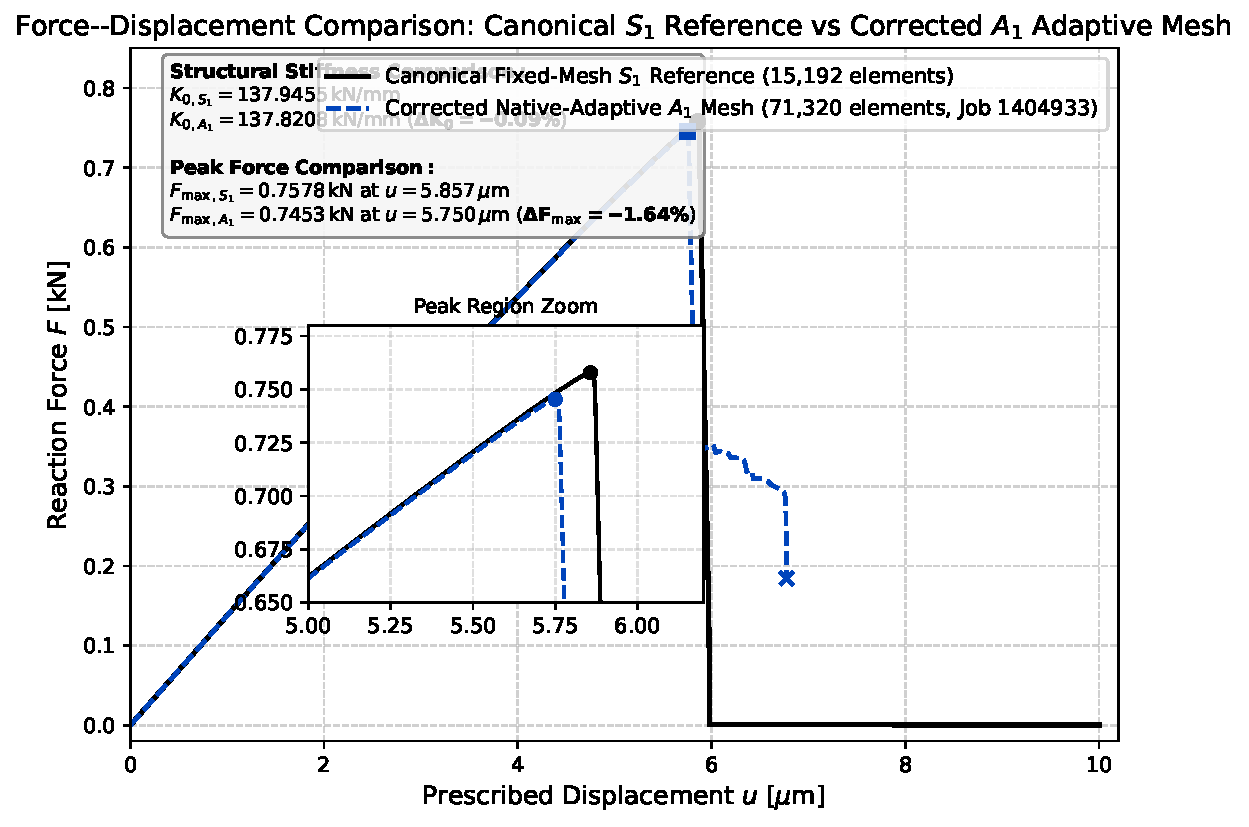
\includegraphics[width=0.82\textwidth]{fig_mode1_fu_recovery.pdf}
  \caption{Force--displacement comparison between the canonical fixed-mesh $S_1$ reference ($15{,}192$ finite elements) and the corrected native-adaptive $A_1$ model with \texttt{errorTarget = 1\%} ($71{,}320$ finite elements). The initial structural stiffness differs by only $0.09\%$, while the adaptive peak reaction force is approximately $1.64\%$ below the reference value.}
  \label{fig:mode1_fu_recovery_pack}
  \figureconclusion{Correcting \texttt{N\_BOTTOM} restores the adaptive model's elastic stiffness. The remaining peak-force difference is therefore a fracture/discretization effect, not evidence of an unresolved elastic boundary-condition defect.}
\end{figure}
